\documentclass{article}[a4paper]
\usepackage[a4paper, left=2.5cm,right=2cm,top=2.5cm,bottom=2.5cm]{geometry}
\usepackage[utf8]{inputenc}
\usepackage{csquotes}
\usepackage{booktabs}
\usepackage{amsmath}
\usepackage{mathtools}% http://ctan.org/pkg/mathtools
\usepackage{caption}
\captionsetup{width=.75\textwidth}
\usepackage[usestackEOL]{stackengine}
\usepackage{float}
\usepackage{subcaption}
\usepackage{tikz}
\usetikzlibrary{shapes.geometric,arrows,positioning,fit}
\usetikzlibrary{shapes,calc,arrows}
\usepackage{natbib}
\usepackage{graphicx}
\usepackage{subfiles}
\usepackage{blindtext}
\usepackage{hyperref}
\usepackage{float}
\def\XXX#1{\textcolor{red}{XXX #1}}
\newcommand{\vect}[1]{\boldsymbol{#1}}
\title{Exercise Sheet 2}
\author{ Bernadeta Griciūtė (7007672)\\
            Zena Al Khalili (7009151)\\
            Sangeet Sagar (7009050\\
            \texttt{\{begr00001,zeal00001,sasa00001\}@stud.uni-saarland.de}
}
\date{\today}
% \pgfplotsset{compat=1.17}
\begin{document}

\maketitle
%#################################################################
\section*{Exercise 2.1 - Eigenvalue decomposition \& SVD }
\subsubsection*{(a)}
We know that  

\begin{flalign*}
    % \vect{Av} = \vect{av} = -2 \begin{bmatrix} 0.6 \\ 0.8 \end{bmatrix} = \begin{bmatrix} -1.2 \\ -1.6 \end{bmatrix} \\
    % \vect{Aw} = \vext{bw} = 0 \begin{bmatrix} 0.8 \\ -0.6  \end{bmatrix} = \begin{bmatrix} 0 \\ 0 \end{bmatrix}
    \vect{Av} = av = -2 \begin{bmatrix} 0.6 \\ 0.8 \end{bmatrix} = \begin{bmatrix} -1.2 \\ -1.6 \end{bmatrix} \\
    \vect{Aw} = aw = 0 \begin{bmatrix} 0.8 \\ -0.6  \end{bmatrix} = \begin{bmatrix} 0 \\ 0 \end{bmatrix}
\end{flalign*}


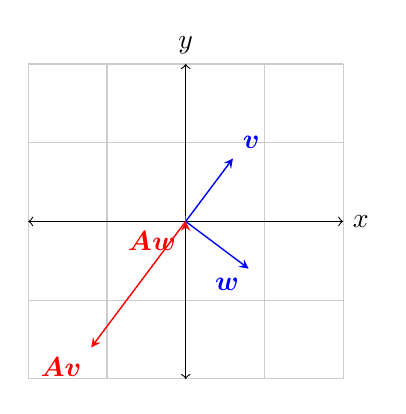
\begin{tikzpicture}
  \draw[thin,gray!40] (-2,-2) grid (2,2);
  \draw[<->] (-2,0)--(2,0) node[right]{$x$};
  \draw[<->] (0,-2)--(0,2) node[above]{$y$};
  \draw[line width=0.5pt,blue,-stealth](0,0)--(0.6,0.8) node[anchor=south west]{$\vect{v}$};
  \draw[line width=0.5pt,blue,-stealth](0,0)--(0.8,-0.6) node[anchor=north east]{$\boldsymbol{w}$};
    \draw[line width=0.5pt,red,-stealth](0,0)--(-1.2,-1.6) node[anchor=north east]{$\boldsymbol{Av}$};
    \draw[line width=0.5pt,red,-stealth](0,0)--(0,0) node[anchor=north east]{$\boldsymbol{Aw}$};
\end{tikzpicture}
\\
The matrix A causes vector v to stretch and reverse direction, while causes vector w to equal to zero. 

\subsubsection*{(b)}
There are infinite eigenvectors for the eigenvalue $a = -2$. Any multiple of an eigenvector is an eigenvector, which spans the set of eigenvectors.
\\
The general solution 
$\vect{X} = \begin{bmatrix} x_1 \\ x_2 \end{bmatrix} = \begin{bmatrix} cx_2 \\ x_2 \end{bmatrix}$
\begin{flalign*}
x_2 = 0.8 \\
x_1 = cx_2 \\
0.6 = c(0.8) \\
\Rightarrow c = 0.75\\
\vect{X}=\begin{bmatrix}0.75x_2\\x_2 \end{bmatrix}
\end{flalign*}
One such eigenvector is $\begin{bmatrix}1.5\\2 \end{bmatrix}$.

\subsubsection*{(c)}
\[\vect{A}=\vect{V} \cdot \vect{\Lambda} \cdot \vect{V}^{-1}\] 
where $\vect{\Lambda}$  is the diagonal matrix  $(\lambda_1,...,\lambda_n)$  and $\vect{V}$ is the matrix of corresponding eigenvectors. However $\vect{V}$ is an orthogonal Matrix which implies that:\\
\[ \vect{V}^{-1} = \vect{V}^{T}\]
\text and $\vect{V}$ is a symmetric matrix which implies that: $\vect{V} = \vect{V}^{T}$

\[\vect{A}=\vect{V} \cdot \vect{\Lambda} \cdot \vect{V}\] 
$\vect{A} =
    \begin{bmatrix}
       0.6 & 0.8 \\ 
       0.8 & -0.6
    \end{bmatrix}
    \begin{bmatrix}
       -2 & 0 \\ 
       0 & 0
    \end{bmatrix}   
    \begin{bmatrix}
       0.6 & 0.8 \\ 
       0.8 & -0.6
    \end{bmatrix} =
    \begin{bmatrix}
       -0.72 & -0.96 \\ 
       -0.96 & -1.28
    \end{bmatrix}
    $
\subsubsection*{(d)}
\[
\vect{A}^{-1} = 
    \frac{1}{ad-bc}
    \begin{bmatrix}
       d & -b \\ 
       -c & a
    \end{bmatrix}
\]
\[
\vect{V}^{-1} = \frac{1}{-0.36-0.64}
    \begin{bmatrix}
       -0.6 & -0.8 \\ 
       -0.8 & 0.6
    \end{bmatrix}
\]
\[
\vect{V}^{-1} = 
    \begin{bmatrix}
       0.6 & 0.8 \\ 
       0.8 & -0.6
    \end{bmatrix} = \vect{V}
\]
\subsubsection*{(e)}
\textbf{singular matrix} - a square matrix that is not invertible. A matrix is singular if its determinant is 0.\\
\textbf{positive definite} - a symmetric matrix whose eigenvalues are all positive.\\
\textbf{positive semi-definite} - a symmetric matrix whose eigenvalues are all positive or zero valued.\\
\textbf{negative definite} - a symmetric matrix whose eigenvalues are all negative.\\
\textbf{negative semi-definite} a symmetric matrix whose eigenvalues are all negative or zero valued.\\
\\~\\
The matrix $\vect{A}$ is a negative semi-definite matrix because its eigenvalues (-2 and 0) are all negative or zero-valued.
\subsubsection*{(f)}

Singular value decomposition (SVD) is defined for all matrices of size $m \times n$ and can decompose a matrix into several components. It can be used to extract useful information from the matrix unlike eigendecomposition. SVD is used to generalize matrix inversion to non-square matrices. Other applications of SVD include matrix approximation, and determining the rank, range, and null space of a matrix.
\\~\\
We use both eigendecomposition and SVD during principal components analysis (PCA). Apart from that, if the given matrix is symmetric and positive definite, SVD simplifies to eigendecomposition, hence we can use both of these techniques.
% https://www.cc.gatech.edu/~dellaert/pubs/svd-note.pdf

% The SVD lets us discover some of the same information the eigendecomposition reveals, but the SVD is more applicable (every matrix has an SVD, but not every matrix has the eigenvalue decomposition). We can search for SVD when the eigendecomposition is not defined (when a matrix is not square). 
% SVD is used to generalize matrix inversion to non-square matrices.
%############################################################################################
%############################################################################################
\section*{Exercise 2.2 - Principal Component Analysis}
\subsubsection*{(a)}

Centering the data is not a requirement; it does however simplify notation and helps us calculate the covariance matrix- which gives us direction of variability in the sample. Figure~\ref{fig:a}
\begin{figure*}[ht]
  \centering
  \includegraphics[keepaspectratio=true,scale=0.6]{HW2/a.png}
  \caption{\textit{Centered dataset with all principle components marked}}
  \label{fig:a}
\end{figure*}

\subsubsection*{(b)}

Encoding matrix is computed by performing SVD on the covariance matrix (size $n \times n$). This gives us a matrix with all eigenvectors (size $n \times n$) of which we pick out only $k$ eigenvectors. The resulting matrix of size $n \times k$ is the encoding matrix.
Figure~\ref{fig:b}
\begin{figure*}[ht]
  \centering
  \includegraphics[keepaspectratio=true,scale=0.6]{HW2/b.png}
  \caption{\textit{1-D data after encoding}}
  \label{fig:b}
\end{figure*}
\clearpage
\subsubsection*{(c)}
The Decoding Matrix D  contains eigenvectors corresponding to the largest eigenvalues of \[ X^{T}X\]
Where X is the design matrix or the Data Matrix, each column of the Data matrix is a training vector. 
Figure~\ref{fig:c}
\begin{figure*}[ht]
  \centering
  \includegraphics[keepaspectratio=true,scale=0.6]{HW2/c.png}
  \caption{\textit{Data in original space after decoding}}
  \label{fig:c}
\end{figure*}

\subsubsection*{(d)}
\ref{fig:d} show a toy data set with tow classes, where pc1 fails to separate the two classes as it's not in the direction of the highest variance.
Figure~\ref{fig:d}
\begin{figure*}[ht]
  \centering
  \includegraphics[keepaspectratio=true,scale=0.6]{HW2/d.png}
  \caption{\textit{Date set in 2-dimensional space}}
  \label{fig:d}
\end{figure*}
\clearpage
since variance is a measure of the "variability" or "spread" of the data, we want our principle components to be in the direction where the data is most separable 
\\
when projecting the data points on pc1 , we notice that we can't separate the one dimensional data into 2 classes.

\begin{figure*}[ht]
  \centering
  \includegraphics[keepaspectratio=true,scale=0.6]{HW2/e.png}
  \caption{\textit{Data projected to pc1}}
  \label{fig:e}
\end{figure*}
\ref{fig:e} shows the data points on pc1. 

%############################################################################################
\section*{Exercise 2.3 - Applications of eigendecomposition in machine learning}
Some of the applications of eigendecomposition are:
\begin{enumerate}
    \item  \textbf{k-means clustering} \cite{Dmitriy:2019} - PCA can be exploited with k-means to viualize high dimensional data such clusters in National health and nutrition survey
    \item \textbf{Linear Discriminant Analysis} \cite{LDA} - LDA, similarly as PCA, is used as dimensionality reduction technique in the pre-processing step for pattern-classification and machine learning applications, but, in contrast to PCA, LDA is “supervised”.
    \item \textbf{Word embeddings} \cite{shin2018interpreting}- eigendecomposition has been used to view word vectors as semantic groups from different domains. 
    \item \textbf{Spectral clustering} \cite{spectral_clustering}- spectral clustering techniques uses eigenvalues of the similarity matrix of the data to perform dimensionality reduction before clustering in fewer dimensions
. 
\end{enumerate}


% %% To cite-\citep{shin2018interpreting}
\bibliographystyle{plain}
\bibliography{references}
\end{document}